\documentclass[11pt, fleqn]{article}

\usepackage{amsmath}
\usepackage{amssymb}
\usepackage[linesnumbered,ruled,vlined]{algorithm2e}
\usepackage{amsthm}
\usepackage{mathtools}
\usepackage{hyperref}
\usepackage{ulem}
\usepackage{enumitem}
\usepackage[left=0.75in, right=0.75in, bottom=0.75in, top=1.0in]{geometry}
\usepackage{floatrow}
\usepackage{float}
\usepackage{graphicx}
\usepackage[export]{adjustbox}
\usepackage{sectsty}
\sectionfont{\centering}
\usepackage{hyperref}
\usepackage[dvipsnames]{xcolor}
\usepackage[perpage]{footmisc}

\usepackage{fancyhdr}
\pagestyle{fancy}
\fancyhf{}
\lhead{190050020 \& 190100044 \& 190100055 \& 190260036}
\rhead{CS 226: Course Project}
\renewcommand{\footrulewidth}{1.0pt}
\cfoot{Page \thepage}

\SetKwInput{KwInput}{Input}                % Set the Input
\SetKwInput{KwOutput}{Output}              % set the Output
\DeclarePairedDelimiter\ceil{\lceil}{\rceil}
\DeclarePairedDelimiter\floor{\lfloor}{\rfloor}
\newtheorem{lemma}{Lemma}

\newcommand{\boxedeq}[2]{\begin{empheq}[box={\fboxsep=6pt\fbox}]{align}\label{#1}#2\end{empheq}}
\setlength{\parindent}{0em}
\renewcommand{\arraystretch}{2}

\title{CS 226: Course Project}
\author{
\begin{tabular}{|c|c|c|c|}
     \hline
     Ankit Kumar Misra & Devansh Jain & Harshit Varma & Richeek Das \\
     \hline
     190050020 & 190100044 & 190100055 & 190260036\\
     \hline
\end{tabular}
}

\date{\today}

\begin{document}

\maketitle
\tableofcontents
\thispagestyle{empty}
\setcounter{page}{0}
\renewcommand{\arraystretch}{1}

\newpage
\section*{Data Paths}
\addcontentsline{toc}{section}{Data Paths}

\subsection*{S0}
\begin{figure}[H]
    \centering
    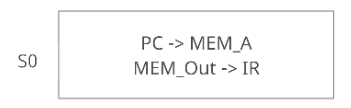
\includegraphics{DataPath/DataPath_S0.PNG}
\end{figure}
\textbf{Control pins}: \\
Register 3 write (IR) \\
MUX 2 select 01 \\

\subsection*{S1}
\begin{figure}[H]
    \centering
    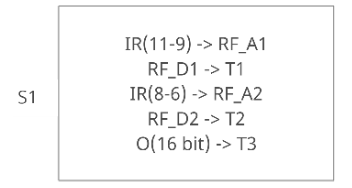
\includegraphics{DataPath/DataPath_S1.PNG}
\end{figure}
\textbf{Control pins}: \\
Register 5 write (T1) \\
Register 6 write (T2) \\
Register 7 write (T3) \\
MUX 6 select 01 \\
MUX 7 select 01 \\
MUX 8 select 0 \\

\subsection*{S2}
\begin{figure}[H]
    \centering
    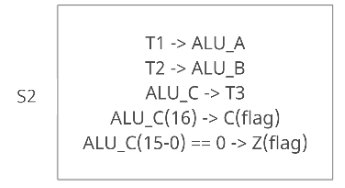
\includegraphics{DataPath/DataPath_S2.PNG}
\end{figure}
\textbf{Control pins}: \\
Register 5 write (T1) \\
MUX 6 select 10 \\
MUX 9 select 10 \\
MUX 10 select 10 \\
if (op\_code is "0000") then alu\_control is 0, carry write, zero write \\
else alu\_control is 1, zero write \\

\subsection*{S3}
\begin{figure}[H]
    \centering
    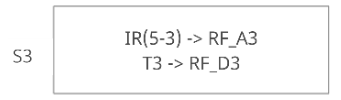
\includegraphics{DataPath/DataPath_S3.PNG}
\end{figure}
\textbf{Control pins}: \\
Register 4 write (RF) \\
MUX 3 select 10 \\
MUX 5 select 11 \\

\subsection*{S4}
\begin{figure}[H]
    \centering
    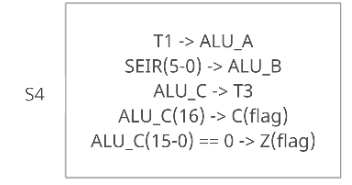
\includegraphics{DataPath/DataPath_S4.PNG}
\end{figure}
\textbf{Control pins}: \\
Register 5 write (T1) \\
MUX 6 select 10 \\
MUX 9 select 01 \\
MUX 10 select 10 \\
carry write, zero write \\

\subsection*{S5}
\begin{figure}[H]
    \centering
    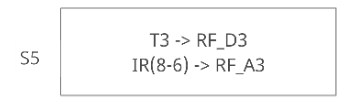
\includegraphics{DataPath/DataPath_S5.PNG}
\end{figure}
\textbf{Control pins}: \\
Register 4 write (RF) \\
MUX 3 select 10 \\
MUX 5 select 11 \\

\subsection*{S6}
\begin{figure}[H]
    \centering
    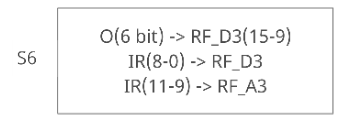
\includegraphics{DataPath/DataPath_S6.PNG}
\end{figure}
\textbf{Control pins}: \\
Register 4 write (RF) \\
MUX 3 select 00 \\
MUX 5 select 01 \\

\subsection*{S7}
\begin{figure}[H]
    \centering
    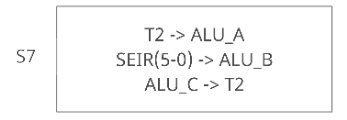
\includegraphics{DataPath/DataPath_S7.PNG}
\end{figure}
\textbf{Control pins}: \\
Register 6 write (T2) \\
MUX 7 select 10 \\
MUX 9 select 01 \\
MUX 10 select 11 \\

\subsection*{S8}
\begin{figure}[H]
    \centering
    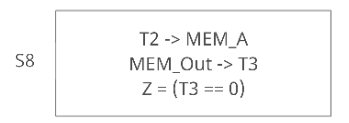
\includegraphics{DataPath/DataPath_S8.PNG}
\end{figure}
\textbf{Control pins}: \\
Register 5 write (T1) \\
MUX 2 select 00 \\
MUX 6 select 00 \\
MUX 11 select 1 \\
zero write \\

\subsection*{S9}
\begin{figure}[H]
    \centering
    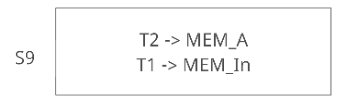
\includegraphics{DataPath/DataPath_S9.PNG}
\end{figure}
\textbf{Control pins}: \\
Register 2 write (MEM) \\
MUX 2 select 00 \\

\subsection*{S10}
\begin{figure}[H]
    \centering
    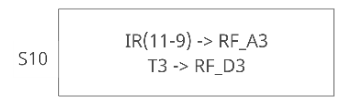
\includegraphics{DataPath/DataPath_S10.PNG}
\end{figure}
\textbf{Control pins}: \\
Register 4 write (RF) \\
MUX 3 select 00 \\
MUX 5 select 11 \\

\subsection*{S11}
\begin{figure}[H]
    \centering
    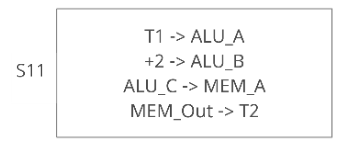
\includegraphics{DataPath/DataPath_S11.PNG}
\end{figure}
\textbf{Control pins}: \\
Register 6 write (T2) \\
Register 7 write (T3) \\
MUX 2 select 11 \\
MUX 7 select 11 \\
MUX 8 select 1 \\
MUX 9 select 11 \\
MUX 10 select 01 \\

\subsection*{S12}
\begin{figure}[H]
    \centering
    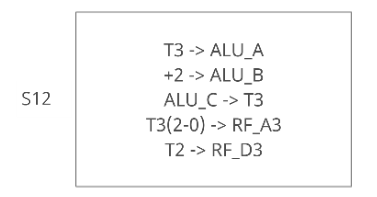
\includegraphics{DataPath/DataPath_S12.PNG}
\end{figure}
\textbf{Control pins}: \\
Register 4 write (RF) \\
Register 5 write (T1) \\
MUX 3 select 11 \\
MUX 5 select 10 \\
MUX 6 select 10 \\
MUX 9 select 11 \\
MUX 10 select 00 \\

\subsection*{S13}
\begin{figure}[H]
    \centering
    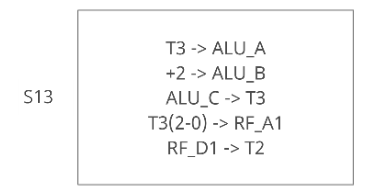
\includegraphics{DataPath/DataPath_S13.PNG}
\end{figure}
\textbf{Control pins}: \\
Register 5 write (T1) \\
Register 6 write (T2) \\
MUX 4 select 1 \\
MUX 6 select 10 \\
MUX 7 select 00 \\
MUX 9 select 11 \\
MUX 10 select 00 \\

\subsection*{S14}
\begin{figure}[H]
    \centering
    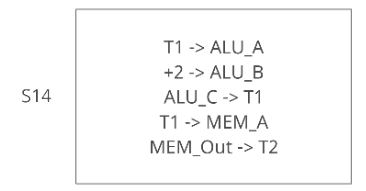
\includegraphics{DataPath/DataPath_S14.PNG}
\end{figure}
\textbf{Control pins}: \\
Register 2 write (MEM) \\
Register 7 write (T3) \\
MUX 2 select 11 \\
MUX 8 select 1 \\
MUX 9 select 11 \\
MUX 10 select 10 \\
MUX 12 select 1 \\

\subsection*{S15}
\begin{figure}[H]
    \centering
    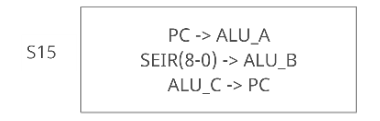
\includegraphics{DataPath/DataPath_S15.PNG}
\end{figure}
\textbf{Control pins}: \\
Register 1 write (PC) \\
MUX 1 select 0 \\
MUX 9 select 00 \\
MUX 10 select 01 \\

\subsection*{S16}
\begin{figure}[H]
    \centering
    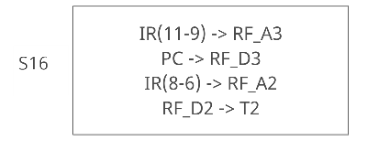
\includegraphics{DataPath/DataPath_S16.PNG}
\end{figure}
\textbf{Control pins}: \\
Register 4 write (RF) \\
Register 6 write (T2) \\
MUX 3 select 00 \\
MUX 5 select 00 \\
MUX 7 select 01 \\

\subsection*{S17}
\begin{figure}[H]
    \centering
    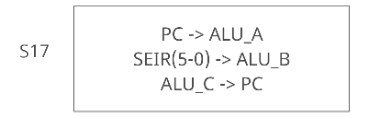
\includegraphics{DataPath/DataPath_S17.PNG}
\end{figure}
\textbf{Control pins}: \\
Register 1 write (PC) \\
MUX 1 select 0 \\
MUX 9 select 01 \\
MUX 10 select 01 \\

\subsection*{S18}
\begin{figure}[H]
    \centering
    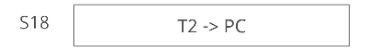
\includegraphics{DataPath/DataPath_S18.PNG}
\end{figure}
\textbf{Control pins}: \\
Register 1 write (PC) \\
MUX 1 select 1 \\

\subsection*{S$_\alpha$}
\begin{figure}[H]
    \centering
    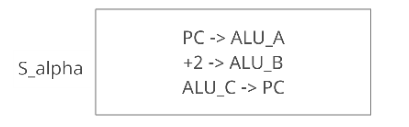
\includegraphics{DataPath/DataPath_S_alpha.PNG}
\end{figure}
\textbf{Control pins}: \\
Register 1 write (PC) \\
MUX 1 select 0 \\
MUX 9 select 11 \\
MUX 10 select 01 \\

\newpage
\section*{State Transition Diagram}
\addcontentsline{toc}{section}{State Transition Diagram}
\begin{figure}[H]
    \centering
    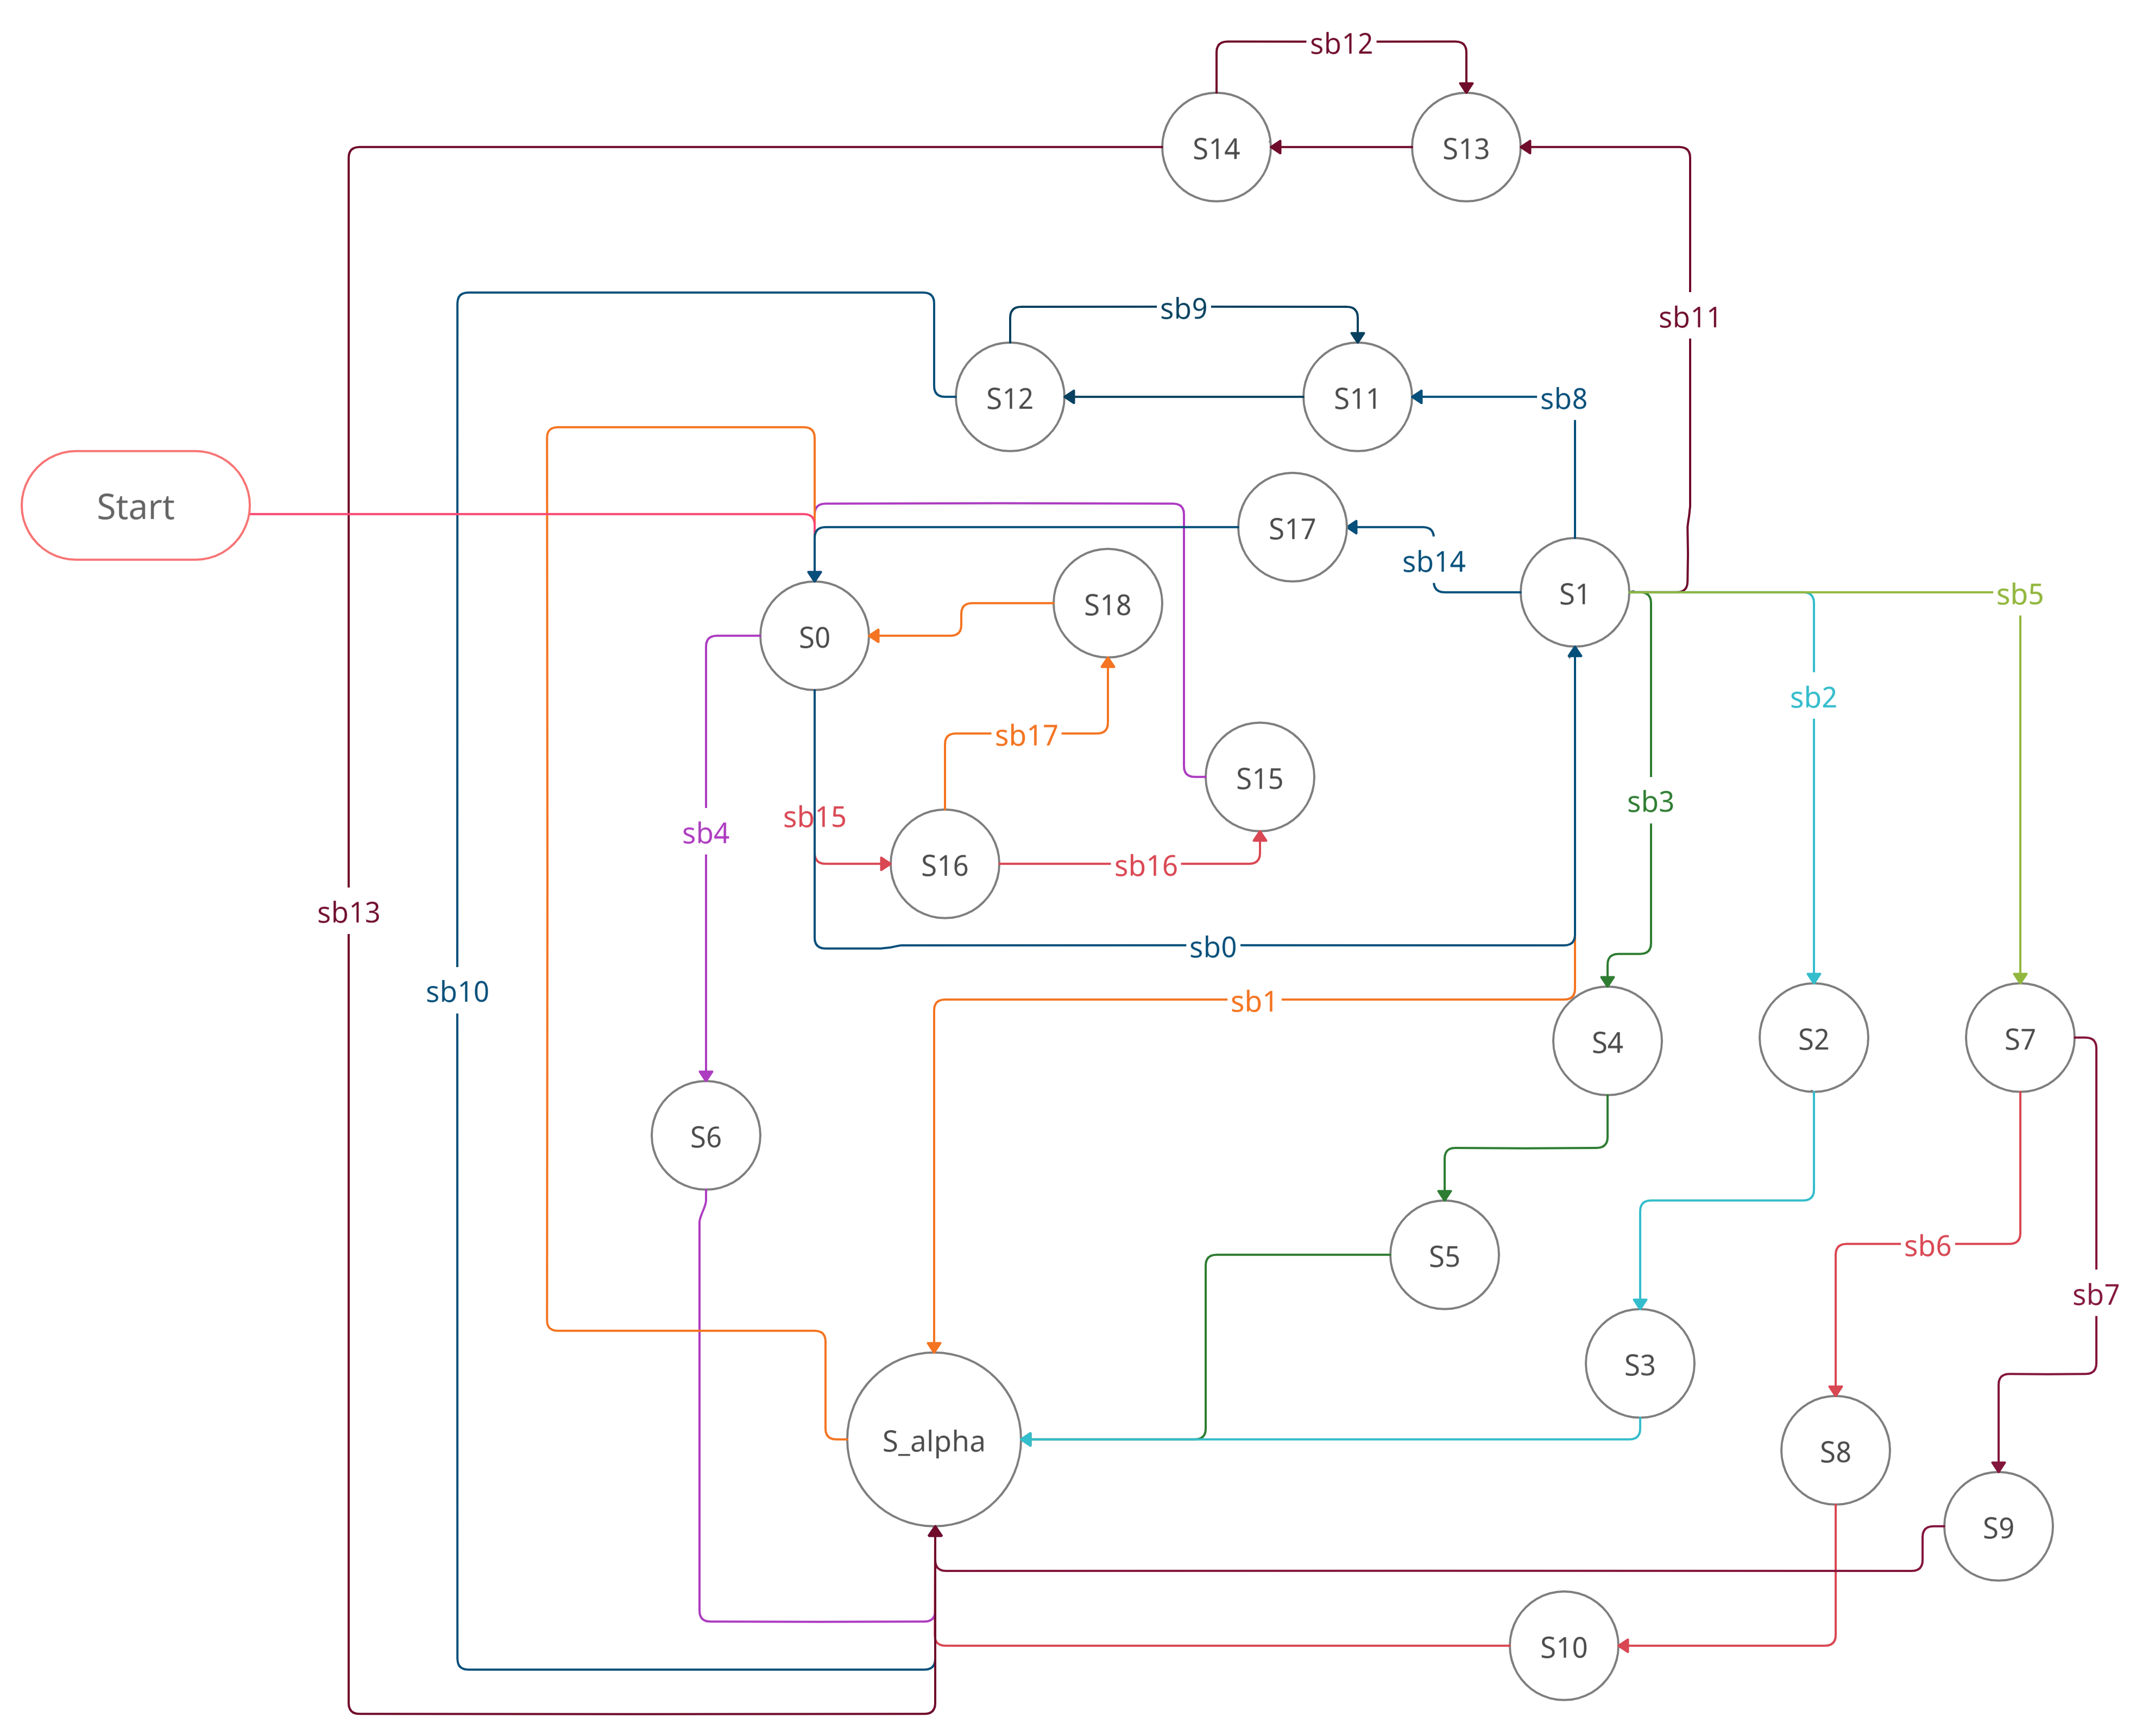
\includegraphics[scale=0.12]{STG.png}
\end{figure}

\textbf{Edge labels:} \\
\texttt{sb0}: OpCode is not (0011 or 1000 or 1001); \\
\texttt{sb1}: [OpCode is (0000 or 0010) with (last two bits are 01 and carry flag unset) or (last two bits are 10 and zero flag unset)] or [OpCode is 1100 with  RF\_D1 != RF\_D2]; \\
\texttt{sb2}: [OpCode is (0000 or 0010) with (last two bits are 01 and carry flag set) or (last two bits are 10 and zero flag set) or (last two bits are 00)]; \\
\texttt{sb3}: OpCode is 0001; \\
\texttt{sb4}: OpCode is 0011; \\
\texttt{sb5}: OpCode is (0100 or 0101); \\
\texttt{sb6}: OpCode is 0100; \hspace*{2em} \texttt{sb7}: OpCode is 0101; \\
\texttt{sb8}: OpCode is 0110; \\
\texttt{sb9}: T3(2-0) is not 111; \hspace*{2em} \texttt{sb10}: T3(2-0) is 111; \\
\texttt{sb11}: OpCode is 0111; \\
\texttt{sb12}: T3(2-0) is not 111; \hspace*{2em} \texttt{sb13}: T3(2-0) is 111; \\
\texttt{sb14}: OpCode is 1100 with RF\_D1 == RF\_D2; \\
\texttt{sb15}: OpCode is (1000 or 1001); \\
\texttt{sb16}: OpCode is 1000; \hspace*{2em} \texttt{sb17}: OpCode is 1001;

\newpage
\section*{Circuit Diagram}
\addcontentsline{toc}{section}{Circuit Diagram}
\begin{figure}[H]
    \centering
    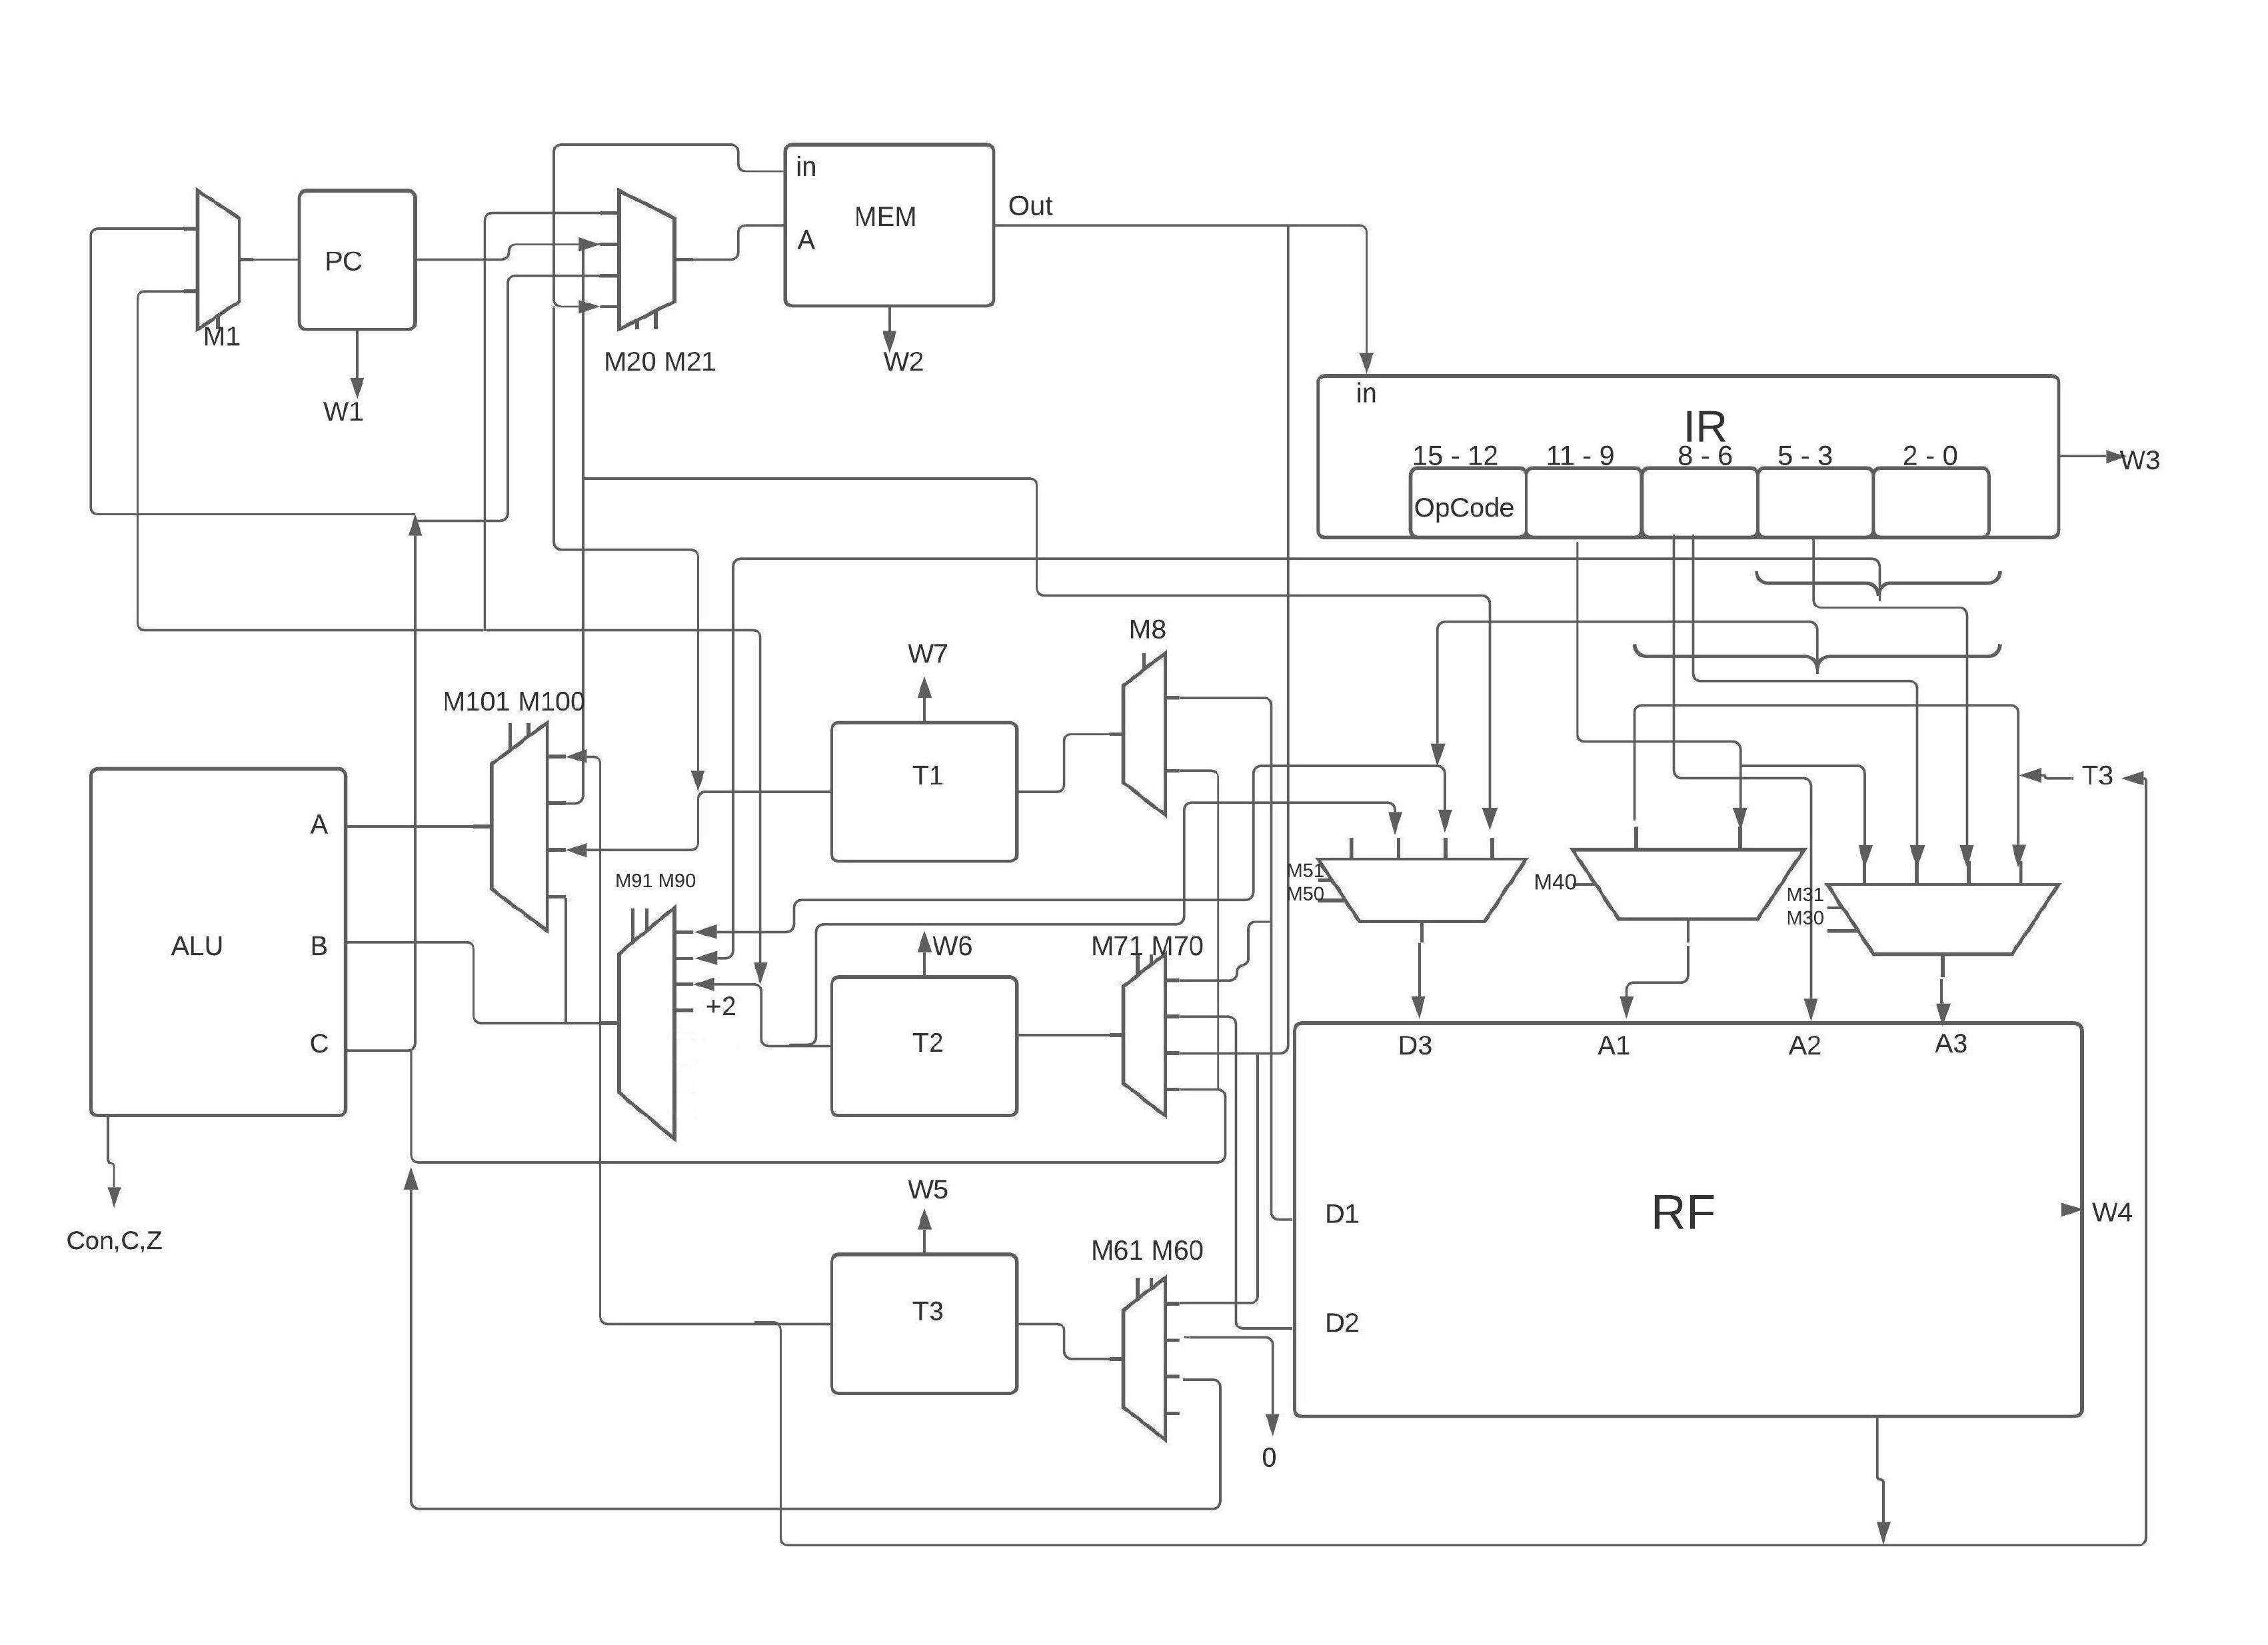
\includegraphics[scale=0.65]{crd.jpeg}
\end{figure}

\newpage
\section*{RTL Viewer}
\addcontentsline{toc}{section}{RTL Viewer}
\begin{figure}[H]
    \centering
    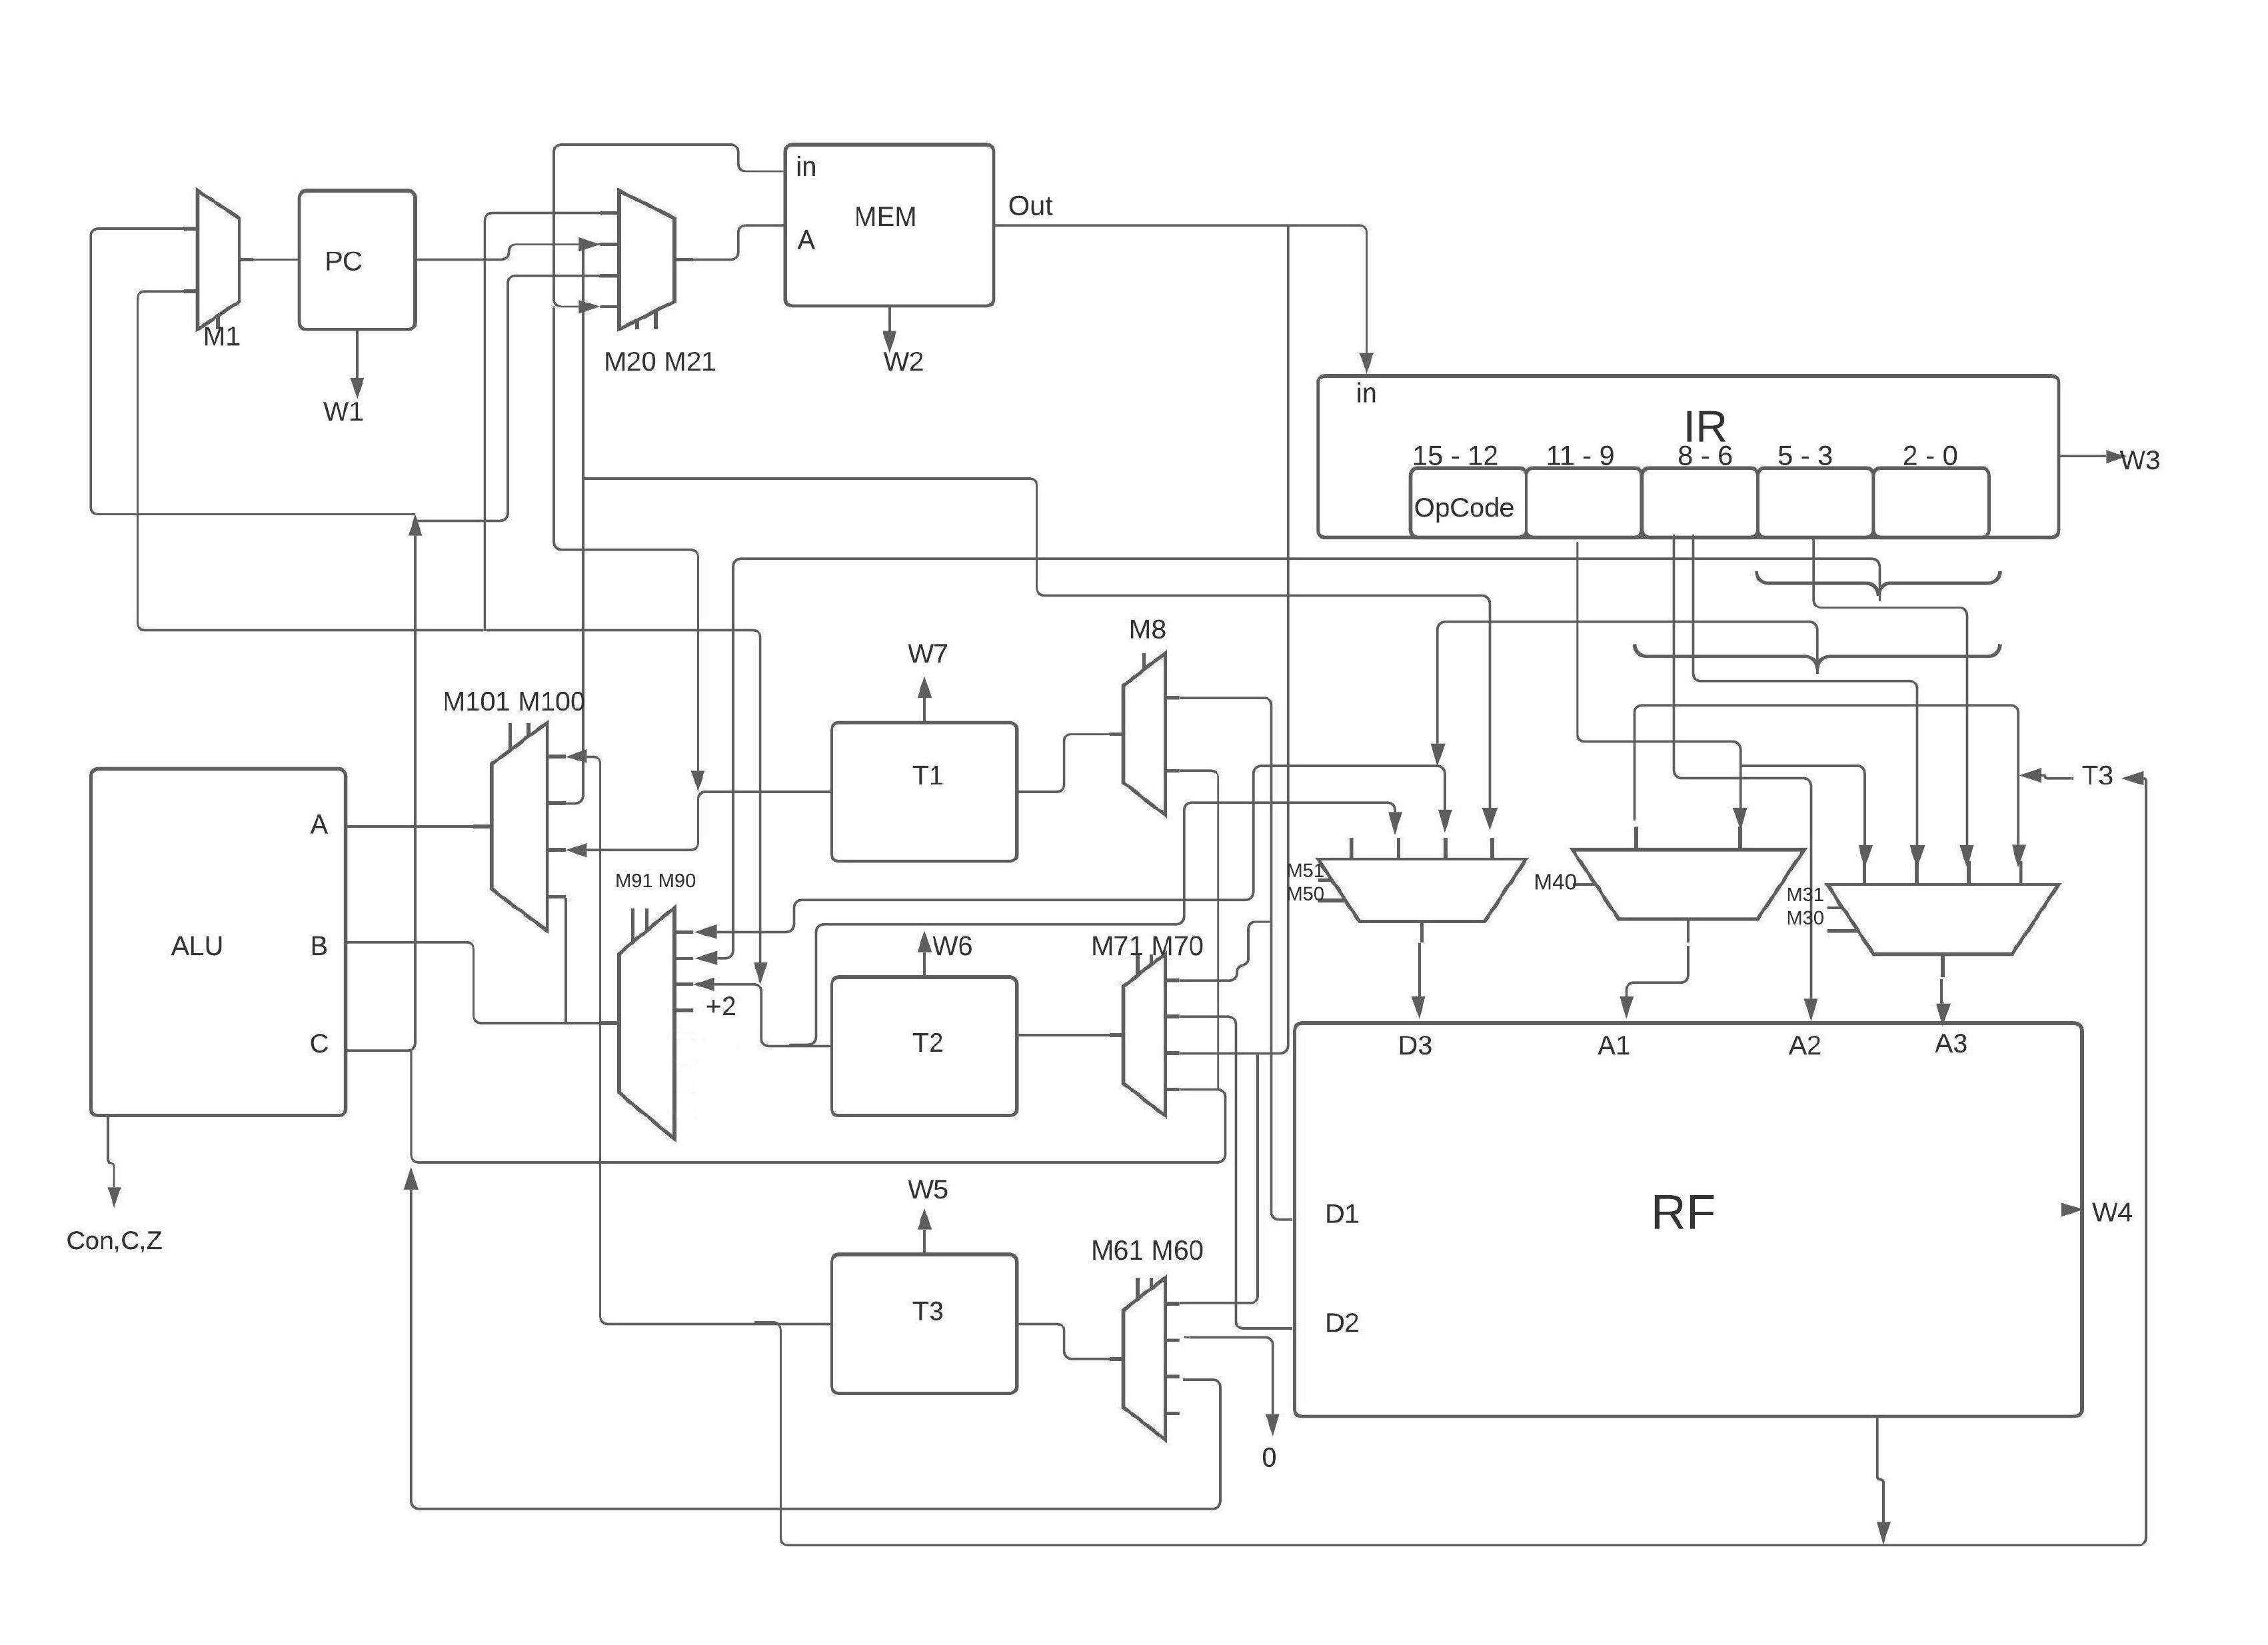
\includegraphics[scale=0.65]{crd.jpeg}
\end{figure}

\newpage
\section*{State Machine Viewer}
\addcontentsline{toc}{section}{State Machine Viewer}
\begin{figure}[H]
    \centering
    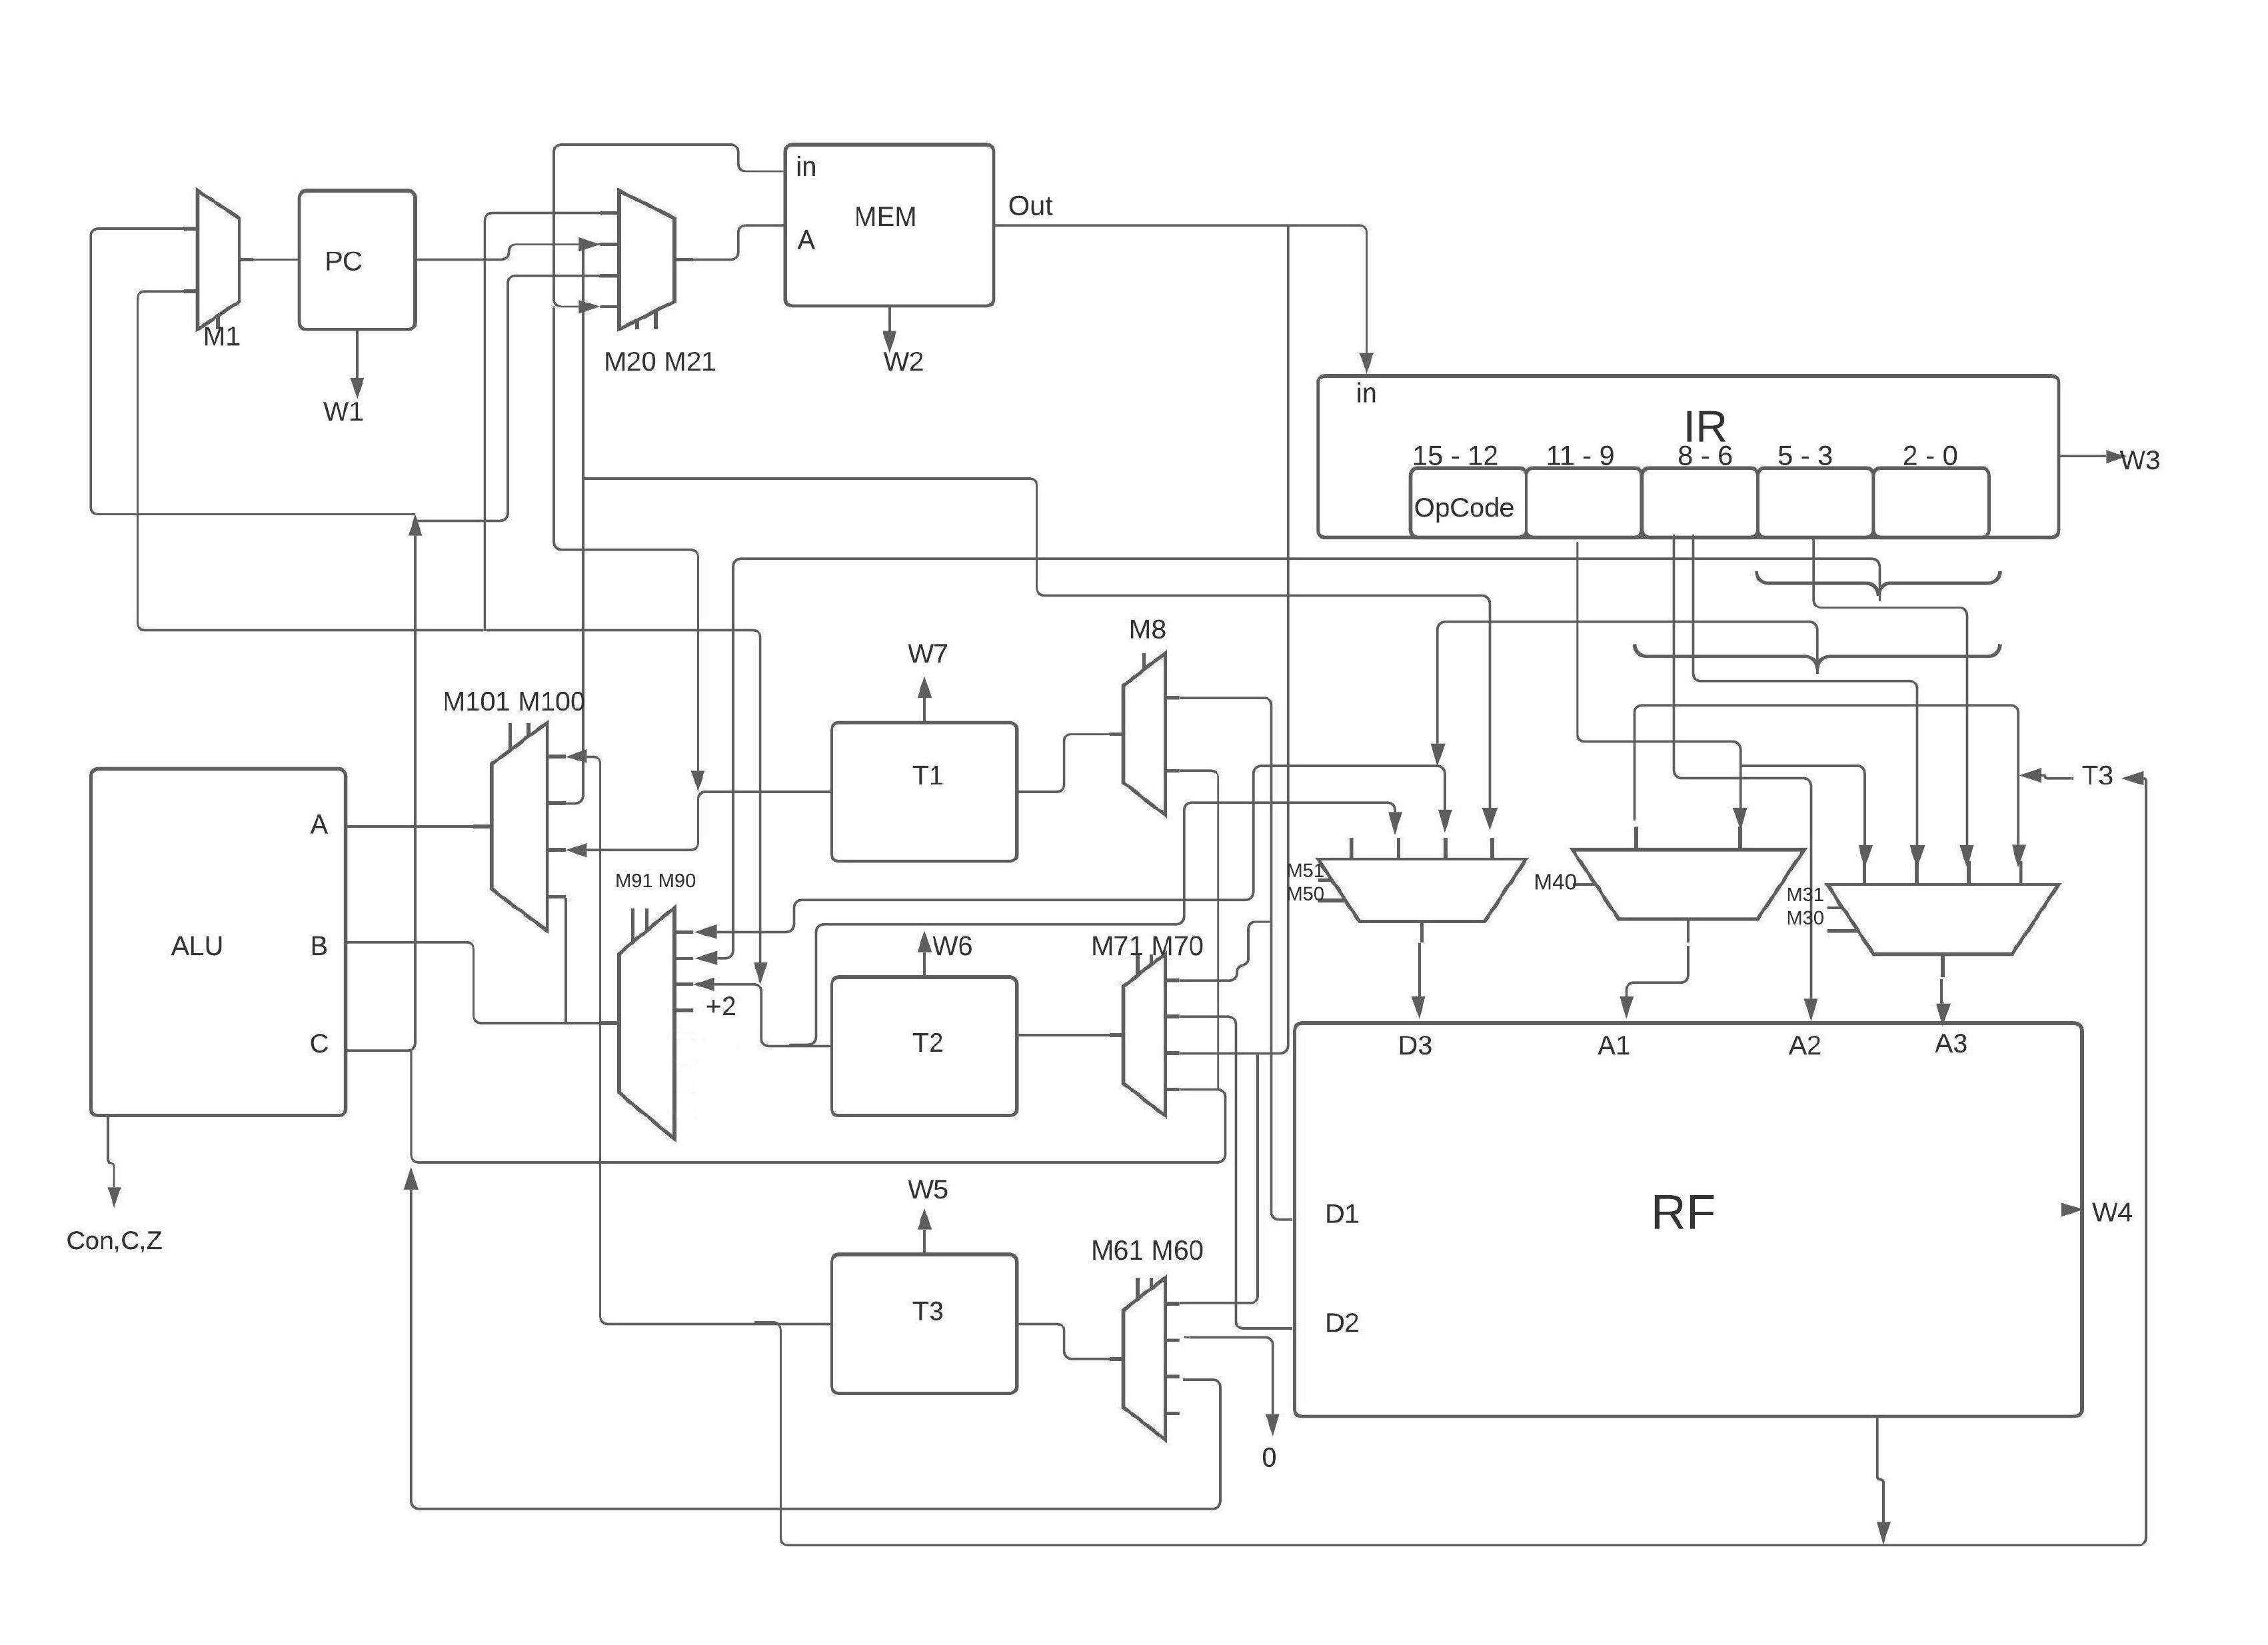
\includegraphics[scale=0.65]{crd.jpeg}
\end{figure}

\end{document}
